\documentclass[12pt]{article}

\usepackage{wrapfig}
\usepackage[spanish]{babel}
\usepackage[utf8]{inputenc}
\usepackage{amsmath}
\usepackage{graphicx}
\usepackage[colorinlistoftodos]{todonotes}

\begin{document}

\begin{titlepage}

\newcommand{\HRule}{\rule{\linewidth}{0.5mm}} % Defines a new command for the horizontal lines, change thickness here

\center % Center everything on the page
 
%----------------------------------------------------------------------------------------
%	HEADING SECTIONS
%----------------------------------------------------------------------------------------

\textsc{\LARGE Universidad de Sonora} \\ [0.4cm]

\includegraphics[scale=.65]{./Images/Logo} \\ [0.3cm]
\textsc{\LARGE Física computacional I}\\[0.3cm]

%----------------------------------------------------------------------------------------
%	TITLE SECTION
%----------------------------------------------------------------------------------------

\HRule \\

{\huge \bfseries Actividad 4\\
Predicción de la marea con la transformada rápida de Fourier\\}

 \HRule \\ [1cm]
\vfill

\begin{minipage}{0.6\textwidth}
	\raggedright
	\large
	\textbf{Gómez García, Manuel Ignacio}
\end{minipage}
~
\begin{minipage}{0.35\textwidth}
	\raggedleft
	\large
	\textbf{10/Diciembre/2018}
\end{minipage}

\end{titlepage}

\section{Introducción}

\noindent Algo que se busca hoy en día es generar una manera de predecir las mareas presentes en una zona con una gran precisión, sin embargo, esto resulta bastante complicado debido a la cantidad de factores que influyen en ello, pero existe otra manera de obtener una aproximación decente de ello, lo cual se basa en el análisis armónico de las ondas que mueven la marea. \\
\indent Como sabemos, la onda que es descrita por el mar no tiene una ecuación sencilla, sino que más bien esta compuesta por diversas ondas armónicas que son las constituyentes de la onda final (la marea), pero ¿cómo es que podemos conocer dichos constituyentes?, ¿qué genera estos movimientos armónicos? pues si bien los factores a analizar serán las posiciones de dos astros bien conocidos, el Sol y la Luna, ya que son factores muy importantes en las mareas presentes sobre la Tierra. \\
\indent Según la alineación de la Tierra con el Sol y la Luna se crean diversas movimientos armónicos que pueden ser diurnos (aproximadamente cada 24 horas), semidiurnos (aproximadamente cada 12 horas) u de otro tipo. De hecho, existen ciertos nombres para los armónicos, de modo que sea más fácil identificar cuáles influyen en cierta zona (figura \ref{fig:constituyentes}).

\begin{figure}[h!]
	\center
	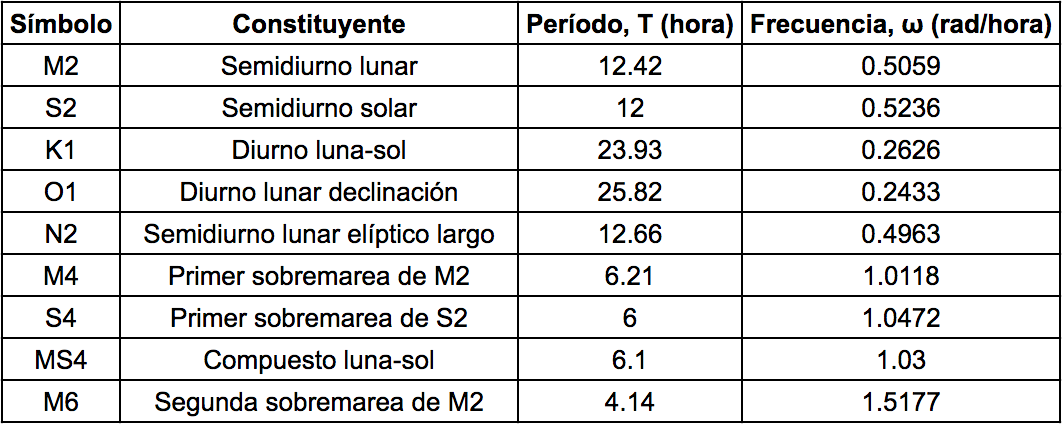
\includegraphics[scale=.3]{./Images/constituyentes}
	\caption{\label{fig:constituyentes} Algunos de los constituyentes existentes \cite{Verde}.}
\end{figure}

\noindent Ahora sólo resta encontrar los constituyentes en nuestra zona de interés en base a los niveles registrados de la marea y para ello haremos uso de la Transformada Rápida de Fourier (FFT, por sus siglas en inglés). Esta función tiene como único requisito que la serie de datos introducidos contenga una cantidad de $2^{n}$ puntos y las ventajas que brinda son bastantes puesto que permite calcular la Transformada de Fourier Discreta (DFT, por sus siglas en inglés) y su inversa, reduce el tiempo de cálculo de $n^{2}$ pasos a $n\cdot log_{2}(n)$, es capaz de resolver ecuaciones de derivadas parciales y algoritmos de multiplicación rápida de grandes enteros, aunque una limitación de esta transformada es que la resolución espectral $\Delta \omega$ es inversamente proporcional al tiempo total $\Delta t$ de recogida de datos en la serie temporal. \\
\indent Haciendo uso de la FFT obtendremos los constituyentes de nuestra zona de estudios, ya que contamos con nuestra serie temporal conteniendo información del nivel del mar a lo largo de cierto tiempo determinado.

\section{Desarrollo}

\noindent Para comenzar, es necesario obtener una serie de datos de alguna estación a orillas del mar. En esta ocasión se utilizará una serie temporal proporcionada por el Centro de Investigación Científica y de Educación Superior de Ensenada (CICESE) \cite{CICESE}, con la cual estaremos trabajando (figura \ref{fig:config}).

\begin{figure}[h!]
	\center
	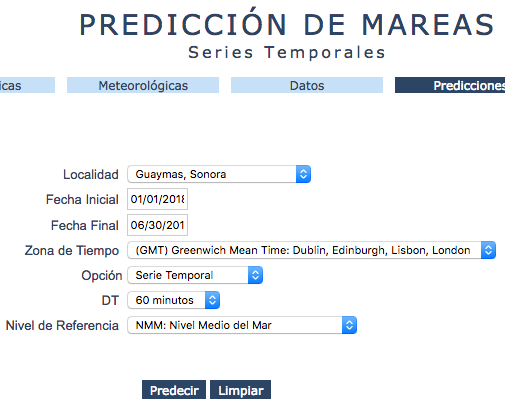
\includegraphics[scale=.67]{./Images/config}
	\caption{\label{fig:config} Ajustes utilizados para la serie de datos.}
\end{figure}

\noindent Haciendo uso de Jupyter Notebook, crearemos un cuadernillo de trabajo Python 3 e importamos las bibliotecas necesarias para el código que estamos por elaborar (figura \ref{fig:bibliotecas}).

\begin{figure}[h!]
	\center
	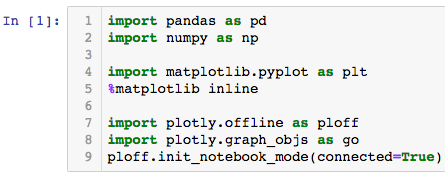
\includegraphics[scale=.6]{./Images/bibliotecas}
	\caption{\label{fig:bibliotecas} Importación de bibliotecas necesarias.}	
\end{figure}

\noindent Ahora procesaremos los datos para tener un mejor manejo de ellos, para esto será necesario agregar, renombrar, ordenar, eliminar y modificar algunas de las columnas con las que ya contamos (figura \ref{fig:process}).

\begin{figure}[h!]
	\center
	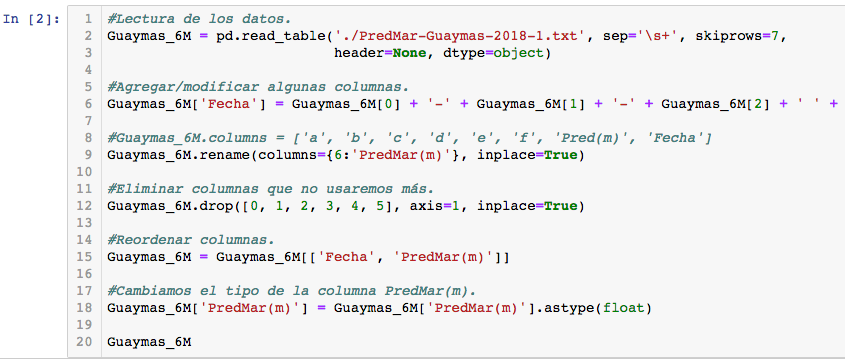
\includegraphics[scale=.6]{./Images/procesamientoA}
	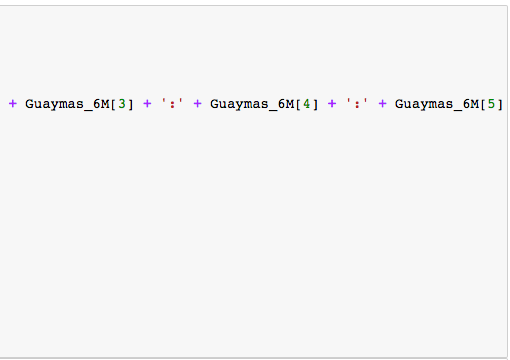
\includegraphics[scale=.6]{./Images/procesamientoB}
	\caption{\label{fig:process} Procesamiento completo aplicado a los datos empleados.}
\end{figure}

Una vez procesados los datos, haremos una gráfica en Plotly para visualizar los valores registrados del nivel del mar, de esta manera podremos darnos una idea del movimiento (figura \ref{fig:cod-nivel-mar}).

\begin{figure}[h!]
	\center
	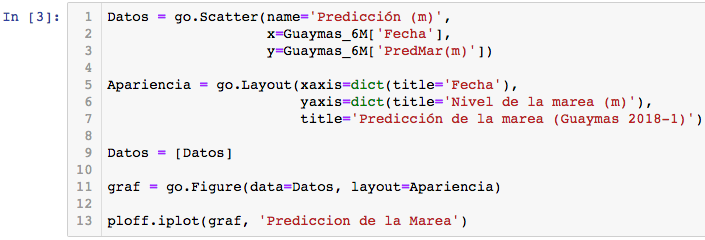
\includegraphics[scale=.6]{./Images/cod-nivel-mar}
	\caption{\label{fig:cod-nivel-mar} Configuración empleada para generar el gráfico en Plotly.}
\end{figure}

Tras correr el código mostrado anteriormente, una gráfica será generada justo debajo del bloque de código (figura \ref{fig:graf-nivel-mar}).

\begin{figure}[h!]
	\center	
	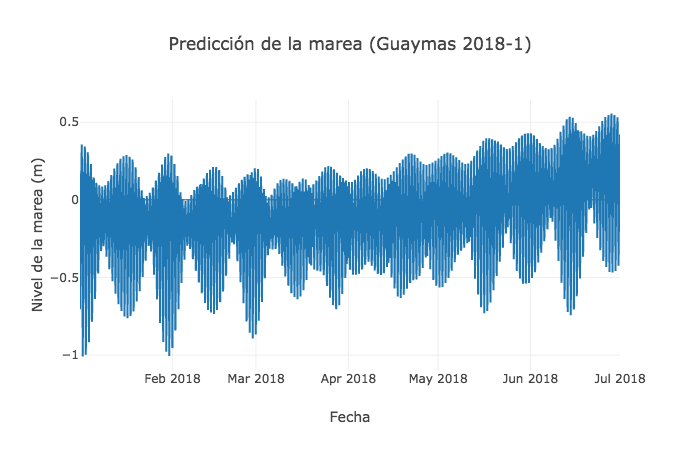
\includegraphics[scale=.6]{./Images/graf-nivel-mar}
	\caption{\label{fig:graf-nivel-mar} Nivel de la marea para Guaymas.}
\end{figure}

Crearemos 3 marcos de datos distintos para analizar en distintas magnitudes la marea y buscar constituyentes con frecuencias menores o mayores (figura \ref{fig:nuevosdf}).

\begin{figure}[h!]
	\center
	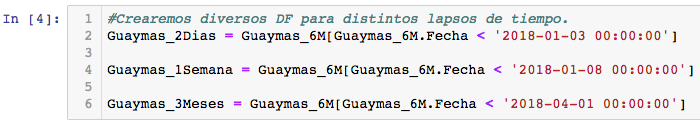
\includegraphics[scale=.6]{./Images/nuevosdf}
	\caption{\label{fig:nuevosdf} Analizaremos 3 lapsos de tiempo distintos para obtener una vista más amplía del fenómeno.}
\end{figure}

Una vez generados los marcos de datos para cada lapso por analizar, procedemos con el código y la gráfica de cada uno de ellos.

\subsection{Marea de Guaymas durante 2 días}

\noindent • Código (figura \ref{fig:cod-2d}) \\

\begin{figure}[h!]
	\center
	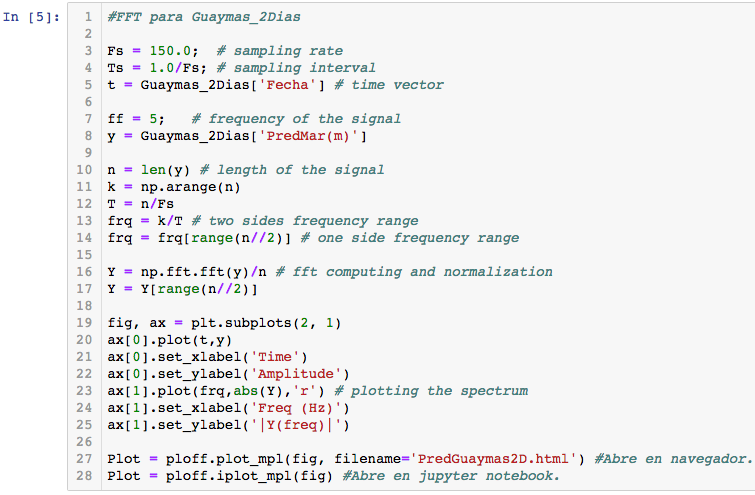
\includegraphics[scale=.6]{./Images/cod-2d}
	\caption{\label{fig:cod-2d} Código para el análisis durante 2 días.}
\end{figure}

\noindent • Gráfica (figura \ref{fig:graf-2d}) \\

\begin{figure}[h!]
	\center
	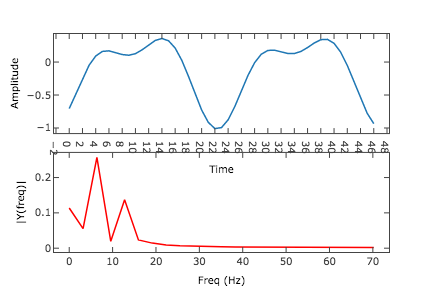
\includegraphics[scale=.6]{./Images/graf-2d}
	\caption{\label{fig:graf-2d} Gráfica para el análisis durante 2 días.}
\end{figure}

\subsection{Marea de Guaymas durante 1 semana}

\noindent • Código (figura \ref{fig:cod-1s}) \\

\begin{figure}[h!]
	\center
	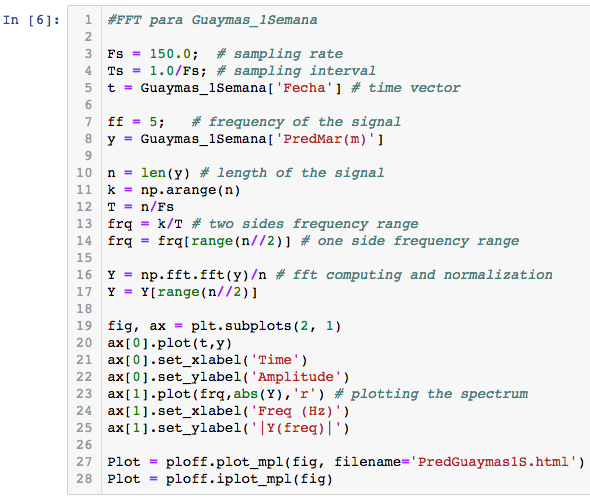
\includegraphics[scale=.6]{./Images/cod-1s}
	\caption{\label{fig:cod-1s} Código para el análisis durante 1 semana.}
\end{figure}

\noindent • Gráfica (figura \ref{fig:graf-1s}) \\

\begin{figure}[h!]
	\center
	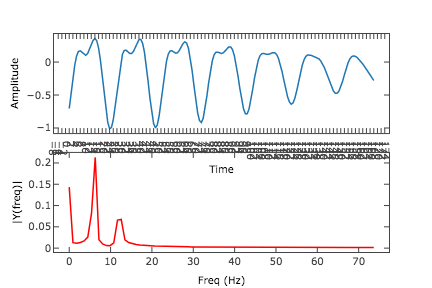
\includegraphics[scale=.6]{./Images/graf-1s}
	\caption{\label{fig:graf-1s} Gráfica para el análisis durante 1 semana.}
\end{figure}

\subsection{Marea de Guaymas durante 3 meses}

\noindent • Código (figura \ref{fig:cod-3m}) \\

\begin{figure}[h!]
	\center
	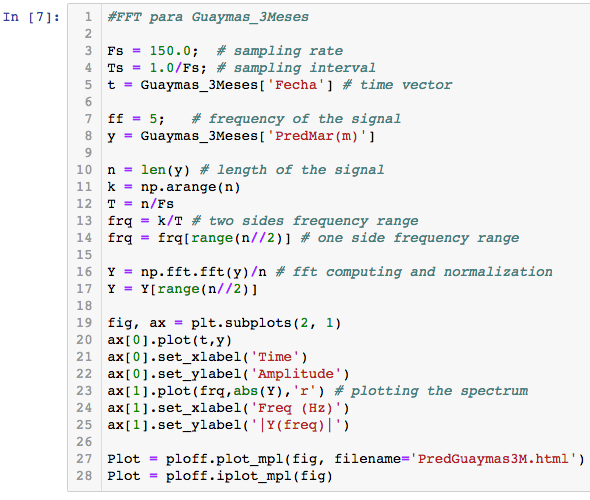
\includegraphics[scale=.6]{./Images/cod-3m}
	\caption{\label{fig:cod-3m} Código para el análisis durante 3 meses.}
\end{figure}

\noindent • Gráfica (figura \ref{fig:graf-3m}) \\

\begin{figure}[h!]
	\center
	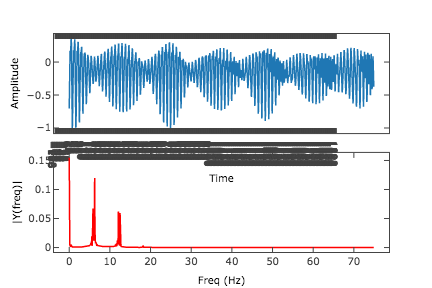
\includegraphics[scale=.6]{./Images/graf-3m}
	\caption{\label{fig:graf-3m} Gráfica para el análisis durante 3 meses.}
\end{figure}

\section{Conclusión}

\noindent Tras ver las gráficas generadas podemos notar como es que se mantiene constante la aparición de ciertos picos que se elevan de manera drástica, los cuales tienen en común la frecuencia en cada uno de los casos que visualizamos, sin embargo, parece ser que la amplitud mostrada en los gráficos disminuye conforme aumentamos el rango de tiempo que abarca cada muestra. \\
\indent Los constituyentes más notorios en la zona podríamos decir que son un semidiurno y una primer sobremarea, de las cuales la sobremarea presenta una mayor amplitud.

\begin{thebibliography}{9}
	\bibitem{NOAA} (2018, Agosto 8). \textsc{Harmonic Analysis}. 10 de diciembre del 2018, de National Oceanic and Atmospheric Administration. Recuperado de https://tidesandcurrents.noaa.gov/harmonic.html
	\bibitem{Giovanni} (2018, Agosto 13). \textsc{Harmonic Analysis and Prediction of Tides}. 12 de diciembre del 2018, de Stony Brook Mathematics Department and Institute for Mathematical Sciences. Recuperado de http://www.math.stonybrook.edu/$\sim$tony/tides/harmonic.html?fbclid=I\\wAR3yu7gX\_cD8MQ52NVjTt-WdWSiHnQbla390IeFimeRvxufgonarBF\\dcCQ4
	\bibitem{Verde} (2018). \textsc{The use of the harmonic analysis method for analysing tidal levels}. 12 de diciembre del 2018, de Ivory Research. Recuperado de https://www.ivoryresearch.com/writers/james-barton-ivory-research-writer/
	\bibitem{Plotly} (2018) \textsc{Fast Fourier Transform in matplotlib}. 10 de diciembre del 2018, de Plotly. Recuperado de https://plot.ly/matplotlib/fft/\#basic-fft-plot-with-matplotlib
	\bibitem{Wiki} (2018, Octubre 21). \textsc{Transformada rápida de Fourier}. 12 de diciembre del 2018, de Wikipedia. Recuperado de https://es.wikipedia.org/wiki/Transformada\_r\%C3\%A1pida\_de\_Fourier
	\bibitem{EHU} (2016). \textsc{Transformada rápida de Fourier (I)}. 12 de diciembre del 2018, de Franco García, Ángel. Recuperado de http://www.sc.ehu.es/sbweb/fisica3/datos/fourier/fourier\_1.html
	\bibitem{CICESE} (2018). \textsc{Predicción de mareas - Series temporales}. 10 de diciembre del 2018, de Centro de Investigación Científica y de Educación Superior de Ensenada (CICESE). Recuperado de http://redmar.cicese.mx/meteoro/graph/prediccion.php
\end{thebibliography}

\end{document}
